%% LyX 2.3.6.1 created this file.  For more info, see http://www.lyx.org/.
%% Do not edit unless you really know what you are doing.
\documentclass[12pt,preprint,3p]{elsarticle}
\usepackage[latin9]{inputenc}
\usepackage{float}
\usepackage{amsmath}
\usepackage{amssymb}
\usepackage{graphicx}

\makeatletter

%%%%%%%%%%%%%%%%%%%%%%%%%%%%%% LyX specific LaTeX commands.
\DeclareTextSymbolDefault{\textquotedbl}{T1}
\floatstyle{ruled}
\newfloat{algorithm}{tbp}{loa}
\providecommand{\algorithmname}{Algorithm}
\floatname{algorithm}{\protect\algorithmname}

%%%%%%%%%%%%%%%%%%%%%%%%%%%%%% User specified LaTeX commands.
%%
%% Copyright 2007, 2008, 2009 Elsevier Ltd
%%
%% This file is part of the 'Elsarticle Bundle'.
%% ---------------------------------------------
%%
%% It may be distributed under the conditions of the LaTeX Project Public
%% License, either version 1.2 of this license or (at your option) any
%% later version.  The latest version of this license is in
%%    http://www.latex-project.org/lppl.txt
%% and version 1.2 or later is part of all distributions of LaTeX
%% version 1999/12/01 or later.
%%
%% The list of all files belonging to the 'Elsarticle Bundle' is
%% given in the file `manifest.txt'.
%%

%% Template article for Elsevier's document class `elsarticle'
%% with numbered style bibliographic references
%% SP 2008/03/01
%%
%%
%%
%% $Id: elsarticle-template-num.tex 4 2009-10-24 08:22:58Z rishi $
%%
%%


%% Use the option review to obtain double line spacing
%% \documentclass[preprint,review,12pt]{elsarticle}

%% Use the options 1p,twocolumn; 3p; 3p,twocolumn; 5p; or 5p,twocolumn
%% for a journal layout:
%% \documentclass[final,1p,times]{elsarticle}
%% \documentclass[final,1p,times,twocolumn]{elsarticle}
%% \documentclass[final,3p,times]{elsarticle}
%% \documentclass[final,3p,times,twocolumn]{elsarticle}
%% \documentclass[final,5p,times]{elsarticle}
%% \documentclass[final,5p,times,twocolumn]{elsarticle}

%% if you use PostScript figures in your article
%% use the graphics package for simple commands
%% \usepackage{graphics}
%% or use the graphicx package for more complicated commands
%% \usepackage{graphicx}
%% or use the epsfig package if you prefer to use the old commands
%% \usepackage{epsfig}

%% The amssymb package provides various useful mathematical symbols
%% The amsthm package provides extended theorem environments
%% \usepackage{amsthm}

%% The lineno packages adds line numbers. Start line numbering with
%% \begin{linenumbers}, end it with \end{linenumbers}. Or switch it on
%% for the whole article with \linenumbers after \end{frontmatter}.
%% \usepackage{lineno}

%% natbib.sty is loaded by default. However, natbib options can be
%% provided with \biboptions{...} command. Following options are
%% valid:

%%   round  -  round parentheses are used (default)
%%   square -  square brackets are used   [option]
%%   curly  -  curly braces are used      {option}
%%   angle  -  angle brackets are used    <option>
%%   semicolon  -  multiple citations separated by semi-colon
%%   colon  - same as semicolon, an earlier confusion
%%   comma  -  separated by comma
%%   numbers-  selects numerical citations
%%   super  -  numerical citations as superscripts
%%   sort   -  sorts multiple citations according to order in ref. list
%%   sort&compress   -  like sort, but also compresses numerical citations
%%   compress - compresses without sorting
%%
%% \biboptions{comma,round}

% \biboptions{}


%\journal{Nuclear Physics B}

\makeatother

\begin{document}

\part{The Numerical Methods}

\section{Finite Element Method}

\subsection{Basic principle of finite element method}

The finite element method (FEM) is a numerical method for the approximate
solution of problems which are described by differential equations.
The practical use of FEM began in the 1950s in construction specially
in the aerospace and car industry. The technique is based on the fact
that the calculation area will be divided into simple sub-areas, the
finite elements. Due to their simple geometry, their physical behavior
can be calculated well with known shape functions. This shape functions
contain parameters that have a physical meaning at a certain point
in component and time. The accuracy of the approximate solution can
be improved by using more parameters, that means smaller elements
or using approach functions of a higher grade. The physical behavior
of the entire body is realized through the transition from one element
to the next element. Since this method requires considerable computing
power, the process thus benefits from the development of powerful
computers.

\subsection{Procedure of the FEM}

To summarize how the finite element method works in general, it will
outline the main steps of the finite element method Element solution
methods listed below \citep{nikishkov_2004}.
\begin{enumerate}
\item Discretion of the calculation domain: The first step is to divide
a solution region into finite elements.
\item Select interpolation functions (shape functions): The second step
is to choose the interpolation function to interpolate the field variables
over the elements.
\item Define the element properties: Set the matrix equation for the finite
elements, which relates the nodal values of the unknown function to
other parameters. The most convenient method is the Galerkin method.
\item Assemble the element equations: It should combine local equations
for all elements which are used for discretization and the boundary
conditions should also be considered.
\item Solve the global equation system: It is a system of linear equations
with a symmetric matrix. For the solution, direct or iterative methods
can be used to find the unknown parameters.
\end{enumerate}

\subsection{Illustration of the method using an example}

It It is considered a simple one-dimensional example to explain the
finite element formulation using Galerkin method. This is about the
principle of using FEM to solve differential equations with boundary
conditions, the extension to higher dimensions is similar and can
be found in the literature\citep{Bathe2016}. The following differential
equation is given

\begin{equation}
a\frac{d^{2}u}{dx^{2}}+b=0,\,\,\,\,\,0\leq x\leq2L
\end{equation}

with Dirichlet and Neuman boundary condition

\begin{align}
 & u\mid_{x=0}=0\\
 & a\frac{du}{dx}\mid_{x=2L}=q\nonumber 
\end{align}

The domain is one-dimensional and consists of two linear elements
and three nodes Fig.\ref{fig:One-dimensional}.
\begin{center}
\begin{figure}[H]
\begin{centering}
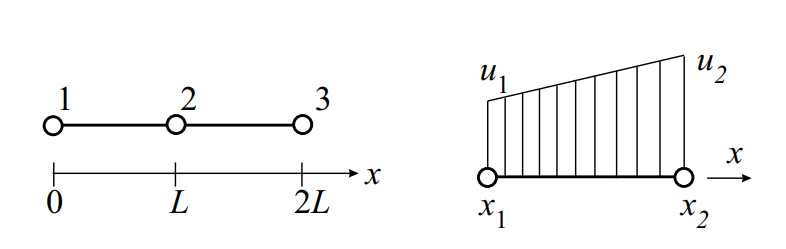
\includegraphics[scale=0.5]{images/Fig1}
\par\end{centering}
\caption{\label{fig:One-dimensional}One-dimensional case with two linear elements
and an interpolation of a function for the domain\citep{nikishkov_2004}}
\end{figure}
\par\end{center}

The approach taken is that the solution can be approximated in this
way

\begin{align}
 & u_{h}\approx u=\underset{i}{\sum N_{i}u_{i}=N_{1}u_{1}+N_{2}u_{2}=\left[N\right]\left\{ u\right\} }\\
 & \left[N\right]=\left[\begin{array}{cc}
N_{1} & N_{2}\end{array}\right]\nonumber \\
 & \left\{ u\right\} =\left\{ \begin{array}{cc}
u_{1} & u_{2}\end{array}\right\} \nonumber 
\end{align}

where $N_{i}$are the shape function and are developed using the Lagrangian
interpolation polynomial

\begin{align}
 & N_{1}=\frac{x-x_{2}}{x_{1}-x_{2}}\\
 & N_{2}=\frac{x-x_{1}}{x_{2}-x_{1}}.\nonumber 
\end{align}

Substituting this into the equation gives us an error called the residual

\begin{equation}
a\frac{d^{2}}{dx^{2}}\left[N\right]\left\{ u\right\} +b=R.
\end{equation}

To minimize the error we use the weighted residuals method and in
the case of Galerkin method for weighting $w$ bis also the shape
function used

\begin{equation}
\int_{\varOmega}w(x)R(x)dx=\int_{x1}^{x2}\left[N\right]^{T}a\frac{d^{2}}{dx^{2}}\left[N\right]\left\{ u\right\} dx+\int_{x1}^{x2}\left[N\right]^{T}bdx=0
\end{equation}

Here is the problem that the second derivative of the linear function
vanishes $\frac{d^{2}}{dx^{2}}\left[N\right]=0.$ The remedy is partial
integration, which leads to a weak formulation of the equation.

\begin{equation}
\int_{x1}^{x2}\left[\frac{dN}{dx}\right]^{T}a\left[\frac{dN}{dx}\right]dx\left\{ u\right\} -\int_{x1}^{x2}\left[N\right]^{T}bdx-\left\{ \begin{array}{c}
0\\
1
\end{array}\right\} a\frac{du}{dx}\mid_{x=x2}+\left\{ \begin{array}{c}
1\\
0
\end{array}\right\} a\frac{du}{dx}\mid_{x=x1}=0
\end{equation}

The whole equation can now be summarized more briefly in matrix and
vector form

\begin{align}
 & \left[K\right]\left\{ u\right\} =\left\{ f\right\} \\
 & \left[K\right]=\int_{x1}^{x2}\left[\frac{dN}{dx}\right]^{T}a\left[\frac{dN}{dx}\right]dx\nonumber \\
 & \left\{ f\right\} =\int_{x1}^{x2}\left[N\right]^{T}bdx+\left\{ \begin{array}{c}
0\\
1
\end{array}\right\} a\frac{du}{dx}\mid_{x=x2}-\left\{ \begin{array}{c}
1\\
0
\end{array}\right\} a\frac{du}{dx}\mid_{x=x1}.\nonumber 
\end{align}

In mechanics, $K$ means the stiffness matrix, $u$ is the displacement
vector and $f$ is the force vector, these terms have become established
in FEM.

For a domain with two elements of length L we get the following matrix
and vector equations

\begin{align}
 & \left[K_{1}\right]=\left[K_{2}\right]=\frac{a}{L}\left[\begin{array}{cc}
1 & -1\\
-1 & 1
\end{array}\right]\\
 & \left\{ f_{1}\right\} =\frac{bL}{2}\left\{ \begin{array}{c}
1\\
1
\end{array}\right\} ,\,\,\,\left\{ f_{2}\right\} =\frac{bL}{2}\left\{ \begin{array}{c}
1\\
1
\end{array}\right\} +\left\{ \begin{array}{c}
0\\
q
\end{array}\right\} .\nonumber 
\end{align}

This two element equation will be assembled because of interact of
the elements in node number 2.

\begin{align}
\left[K\right]\left\{ u\right\}  & =\left[\begin{array}{ccc}
k_{1} & -k_{1} & 0\\
-k_{1} & k_{1}+k_{2} & k_{2}\\
0 & -k_{2} & k_{2}
\end{array}\right]\left\{ \begin{array}{c}
u_{1}\\
u_{2}\\
u_{3}
\end{array}\right\} =\frac{a}{L}\left[\begin{array}{ccc}
1 & -1 & 0\\
-1 & 2 & -1\\
0 & -1 & 1
\end{array}\right]\left\{ \begin{array}{c}
u_{1}\\
u_{2}\\
u_{3}
\end{array}\right\} \\
 & =\left\{ \begin{array}{c}
f_{11}\\
f_{12}+f_{21}\\
f_{22}
\end{array}\right\} =\frac{bL}{2}\left\{ \begin{array}{c}
1\\
2\\
1
\end{array}\right\} +\left\{ \begin{array}{c}
0\\
0\\
q
\end{array}\right\} \nonumber 
\end{align}

Consider the boundary condition the final appearance equation system
is

\begin{equation}
\frac{a}{L}\left[\begin{array}{ccc}
1 & 0 & 0\\
0 & 2 & -1\\
0 & -1 & 1
\end{array}\right]\left\{ \begin{array}{c}
u_{1}\\
u_{2}\\
u_{3}
\end{array}\right\} =\frac{bL}{2}\left\{ \begin{array}{c}
0\\
2\\
1
\end{array}\right\} +\left\{ \begin{array}{c}
0\\
0\\
q
\end{array}\right\} .
\end{equation}

The exact solution and the approximate solution are shown in Fig.\ref{fig:Comparison}
for the Parameters $a=b=q=L=1.$
\begin{center}
\begin{figure}[H]
\begin{centering}
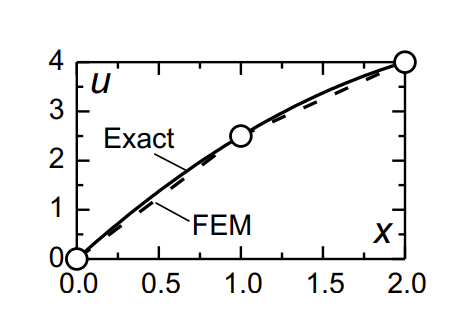
\includegraphics[scale=0.6]{images/Fig2}
\par\end{centering}
\caption{\label{fig:Comparison}Comparison between analytical and numerical
solution\citep{nikishkov_2004}}
\end{figure}
\par\end{center}

All these steps are realized for the models in this work in Comsol
Multiphysics.

\section{Genetic Algorithms}

\subsection{Historical Context and Basics}

Genetic algorithms (GA) are machine learning models and optimization
methods motivated by the evolutionary processes in nature and so the
vocabulary was adopted from genetics. In this method, learning is
understood as competition between evolved species in a population,
and this makes the algorithms directed probability algorithms and
thus much more efficient than random search algorithms. GAs were first
proposed by John Holland in the 1960s and further developed by his
students and colleagues at the University of Michigan in the 1960s
and 1970s \citep{holland1975adaptation}. Genetic algorithms are useful
for many types of complex optimization tasks well suited:
\begin{itemize}
\item No fundamental limitations regarding the function to be optimized,
such as continuity, derivability, etc.
\item Particularly suitable for problems with a very large search space
where an optimal search by listing all possible solutions is no longer
possible.
\item The global extremum is sought and not just the nearest local extremum.
\item Genetic algorithms can be efficiently implemented on parallel computing
structures.
\end{itemize}
One of the weaknesses of the algorithm is that finding the optimal
solution cannot be guaranteed. More information on this topic can
be found in the literature \citep{fogel1997evolutionary}. Algorithm
\ref{alg:Basic-Genetic} shows the basic structure of a GA.

\begin{algorithm}[H]
$t\leftarrow0$

Generate population $P\left(t\right)$ randomly

evaluate fitness for $P\left(t\right)$

\textbf{while} ( \textbf{not} termination condition )

\textbf{do}

$t\leftarrow t+1$

create new population $P\left(t\right)$

select

recombine

mutate

evaluate fitness for$\left(P\left(t\right)\right)$;

\textbf{end while}

\caption{\label{alg:Basic-Genetic}Basic Genetic Algorithm \citep{Buttelmann2004}}
\end{algorithm}

\begin{flushleft}
The GA starts with a randomly generated population (a set of chromosomes)
and the fitness is evaluated by the fitness function. Evolutionary
it means that the fittest in the population survive and mathematically
the fitness function is the function that is trying to optimize the
solution. While the termination condition is not achieved, the GA
performs a fitness based selection, recombination and mutation process
to create a succeeding population and subsequently the next generation.
During recombination, parent chromosomes are selected and their genetic
material is recombined to produce child chromosomes. These then advance
into the next population. As this process is repeated, a sequence
of successive generations develops and the average fitness of the
chromosomes tends to increase until the termination criterion is reached.
\par\end{flushleft}

\subsection{The detailed structure}

A GA consists of a number of different components. This is a special
strength because it means that standard components can be reused in
many different GAs with trivial customization, thus easing implementation\citep{mccall2005genetic}.
The vocabulary for genetic algorithms was taken from genetics.

\subsubsection{Population}

In order to use a genetic algorithm, a solution space must first be
specified. From the solution space an initial population is randomly
generated which is a set of individuals or chromosomes. At this stage
one can apply heuristics to give the algorithm a better starting position.
A chromosome represents a point in the search space and consists of
genes that represent the elements of a solution \ref{fig:Population-gen}.
The number of genes represents a measure of the size of a solution.

\begin{figure}[H]
\centering{}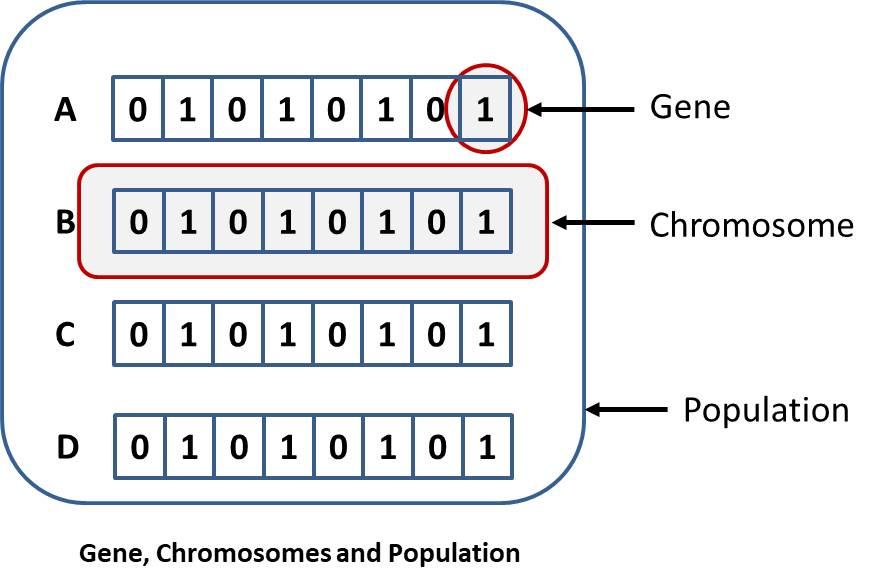
\includegraphics[scale=0.5]{images/Genetic-Algorithm-Illustrated}\caption{\label{fig:Population-gen}Population construction in GA \citep{kindsonthegenius_2020}}
\end{figure}


\subsubsection{Fitness and Objective Function}

The fitness function of an individual $f\left(i_{k}\right)$ in a
population $P=\left\{ i_{1},i_{2},...,i_{n}\right\} $ gives the probability
whether that individual can survive and thus pass on their genes.
Since the fitness function is a positive real number, it is obtained
by scaling from the objective function $f(i)=scale(o(i))$, which
corresponds to the optimization goal of the optimization problem.

\subsubsection{Selection}

The GA uses the selection to appoint individuals for reproduction
as a new generation on the principle of biological evolution ''survival
of the fittest''. Individuals with higher fitness have a greater chance
of selection than those with lower fitness, thus creating selection
pressure on the individuals in the direction of optimal solution.
Choosing the right selection pressure is crucial, if the selection
pressure is too high, the solution converges prematurely to the local
optimum. However, if the selection pressure is too low, the optimal
individuals are hardly favored. Therefore, the solution will either
not converge or will only converge at a much slower rate.

There are several selection methods and the choice is made according
to the task. An example of such a method presented here is the selection
scheme Stochastic Universal Sampling (SUS). In this process each Individual
is assigned a segment on the roulette wheel. The size of the segment
is proportional to fitness of the individual. The wheel is turned
and then $n$ pointers arranged evenly around the wheel choose $n$
individuals for reproduction. A detailed description of the various
selection schemes can be found in Handbook of Evolutionary Computation
\citep{Back:1997:HEC:548530}.

\subsubsection{Crossover}

The crossover operator allows mixing of genetic material from selected
initial chromosomes to create offspring chromosomes. After selecting
two parent chromosomes for recombination, a random number is generated
in the interval $[0,1]$ with uniform probability and compared with
a predetermined \textquotedbl crossover rate\textquotedbl . If the
random number is greater than the crossover rate, no crossover occurs
and one or both parents will proceed unchanged to the next level or
recombination. If the crossover rate is greater than or equal to the
random number, the crossover operator is applied Fig \ref{fig:Uniform-crossover-for}.
There are many other ways to perform the crossover, see the following
literature \citep{Hasanebi2000}.

\begin{figure}[H]
\centering{}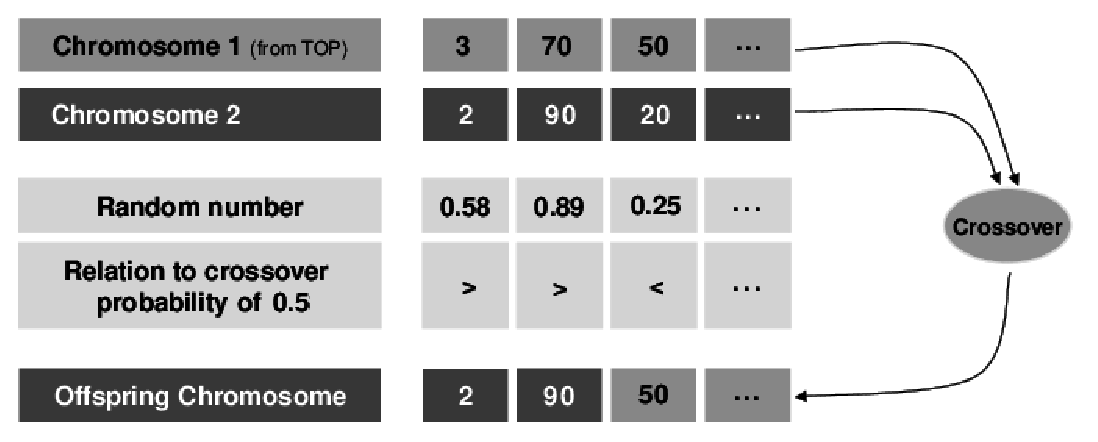
\includegraphics[scale=0.6]{images/Example-of-parameterized}\caption{\label{fig:Uniform-crossover-for}Uniform crossover for crossover
rate of $0.5$ \citep{article1}}
\end{figure}


\subsubsection{Mutation}

The mutation operator works much like the crossover operator Fig.\ref{fig:Mutation-in-gene}.
It changes the genes values with less probability $p_{\textrm{m}}$
and so the solution in smaller step \citep{Buttelmann2004}.

\begin{figure}[H]
\begin{centering}
\textbf{Before the mutation:}
\par\end{centering}
\begin{centering}
Chromosome one: $\left[\begin{array}{ccccccccccc}
4 & 50 & 10 & 7 & 9 & 60 & 7 & 600 & 0.9 & 3 & 340\end{array}\right]$
\par\end{centering}
\begin{centering}
\textbf{After the mutation:}
\par\end{centering}
\begin{centering}
Chromosome one: $\left[\begin{array}{ccccccccccc}
4 & 90 & 10 & 7 & 9 & 60 & 7 & 1000 & 0.9 & 3 & 340\end{array}\right]$
\par\end{centering}
\caption{\label{fig:Mutation-in-gene}Mutation in gene number 2 and 8}
\end{figure}

\begin{flushleft}
The idea is not to get stuck in local minima but , through this method,
to reach the global minima.The chosen values for the mutation probability
pm are usually 0.01 or 0.001. Some sources \citep{muhlenbein1992genetic}
prefer the chromosome length $L$ depended mutation probability as
the optimal probability $p_{\textrm{mopt}}=1/L$, which is used for
this implementation.
\par\end{flushleft}

\subsubsection{Termination}

For the termination of GA there is a criterion needed. Therefore there
are several possibilities like time constraints \citep{kramer2017genetic}
or the consideration of convergence. Another popular variant used
for this implementation is a certain number of generations.

\bibliographystyle{bibtex-daten/unsrtdin}
\bibliography{bibtex-daten/bachelorarbeit-info}

\end{document}
